\documentclass{article}
\usepackage[frenchb]{babel}
\usepackage[utf8]{inputenc}
\usepackage[T1]{fontenc}
\usepackage{graphicx}
\usepackage{fancyhdr}

\pagestyle{fancy}
\title{Projet programmation par contrainte : Elisabeth}
\author{}


\begin{document}

\maketitle
\date


\begin{figure}[h]

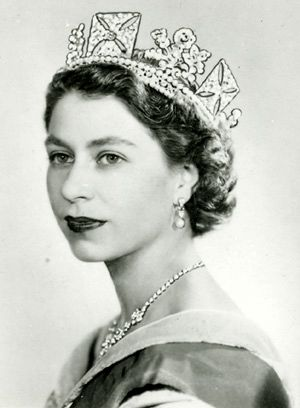
\includegraphics[width = 250px]{./picture/eli.jpg}


\end{figure}




\newpage


\tableofcontents

\newpage

\section{Introduction}

\vspace{1cm}

\subsection{Problématique et but du projet}

\vspace{1cm}

Le but de ce projet TP est d'implementer un solveur pour des domaines CPSs finis.
La conception de ce projet s'entends sur trois séances de TP et dois nous permettre de résoudre le problème des dammes aux échecs.

Il y a un systeme de n case avec n dame mais chaque dame doit être placé de façon à ce qu'elles ne puissent s'attaquer à une autre.

Nous avons décidé d'utiliser python 3.5.1 comme language de programmation. 

\vspace{1cm}




\subsection{Notre groupe}

\vspace{1cm}

\begin{tabbing}


\=blaaaaaaaaaa	\=bmaaaaaaaaaaaaaaaaa		\=baaaaaaa\kill \\
\>Thibault 	\>Béziers La fosse		\>M1ALMA\\
\>Dennis	\>Bordet			\>M1ALMA\\
\>Joachim	\>Clayton			\>M1ALMA\\
\>Alexis	\>Giraudet			\>M1ALMA\\
\>Benjamin 	\>Moreau			\>M1ALMA\\


\end{tabbing}

\vspace{1cm}
\section{Code???}
\vspace{2cm}


blablabla

\vspace{1cm}
\section{Section2}
\vspace{2cm}


blabalabalababal


\vspace{1cm}
\section{Conclusion}
\vspace{2cm}


\end{document}
